% !TEX encoding = UTF-8 Unicode.

% Based on https://github.com/Miracle0565/BUCT-Beamer-Theme

\documentclass[
10pt,
aspectratio=43,
]{beamer}
\setbeamercovered{transparent=10}
\usetheme[
%  showheader,
%  red,
  purple,
%  gray,
%  graytitle,
  colorblocks,
%  noframetitlerule,
]{Verona}

\usepackage[T1]{fontenc}
\usepackage{tikz}
\usepackage[utf8]{inputenc}
\usepackage{lipsum}
%%%%%%%%%%%%%%%%%%%%%%%%%%%%%%%
% Mac上使用如下命令声明隶书字体,windows也有相关方式,大家可自行修改
\providecommand{\lishu}{\CJKfamily{zhli}}
%%%%%%%%%%%%%%%%%%%%%%%%%%%%%%%
\usepackage{tikz}
\usetikzlibrary{fadings}
%
%\setbeamertemplate{sections/subsections in toc}[ball]
\usepackage{xeCJK}
\usepackage{listings}
\usepackage{caption}
\usepackage{subfigure}
\usefonttheme{professionalfonts}
\def\mathfamilydefault{\rmdefault}
\usepackage{amsmath}
\usepackage{multirow}
\usepackage{booktabs}
\usepackage{bm}
\setbeamertemplate{section in toc}{\hspace*{1em}\inserttocsectionnumber.~\inserttocsection\par}
\setbeamertemplate{subsection in toc}{\hspace*{2em}\inserttocsectionnumber.\inserttocsubsectionnumber.~\inserttocsubsection\par}
\setbeamerfont{subsection in toc}{size=\small}
\AtBeginSection[]{%
	\begin{frame}%
		\frametitle{Outline}%
		\textbf{\tableofcontents[currentsection]} %
	\end{frame}%
}

\AtBeginSubsection[]{%
	\begin{frame}%
		\frametitle{Outline}%
		\textbf{\tableofcontents[currentsection, currentsubsection]} %
	\end{frame}%
}

\title{高等数学C}
%\subtitle{A Simple while elegant template}
\author[P.Yu]{余沛}
\mail{peiy\_gzgs@qq.com}
\institute[Guangzhou College of Technology and Business]{Guangzhou College of Technology and Business \\
  广州工商学院}
\date{\today}
\titlegraphic[width=4cm]{logo.png}{}




%%%%%%%%%%%%%%%%%%%%%%%%%%%%%%%%
% ----------- 标题页 ------------
%%%%%%%%%%%%%%%%%%%%%%%%%%%%%%%%



\begin{document}

\maketitle

%%% define code
\defverbatim[colored]\lstI{
	\begin{lstlisting}[language=C++,basicstyle=\ttfamily,keywordstyle=\color{red}]
	int main() {
	// Define variables at the beginning
	// of the block, as in C:
	CStash intStash, stringStash;
	int i;
	char* cp;
	ifstream in;
	string line;
	[...]
	\end{lstlisting}
}
%%%%%%%%%%%%%%%%%%%%%%%%%%%%%%%%
% ----------- FRAME ------------
%%%%%%%%%%%%%%%%%%%%%%%%%%%%%%%%

\begin{frame}
	\frametitle{求最大容积}
	\everymath{\displaystyle}
	\begin{block}{问题}
		将边长为 $a$ 的正方形铁皮, 四角各截去相同的小正方形, 折成一个无盖方盒, 问如何截, 使方盒的容积最大?最大值为多少?
	\end{block}
	\pause
	\begin{block}{}
		设小正方形的边长为 $x$, 则方盒的容积为
		\[ V = x(a-2x)^2, \quad x \in \left(0, \frac{a}{2}\right) \]
	\end{block}
	\pause
	\begin{block}{}
		求导得 $V' = (a-2x)(a-6x)$, 得唯一驻点 $x = \frac{a}{6}$. 导数在驻点左侧为正, 右侧为负, 所以 $x = \frac{a}{6}$ 为极大值点, 即为最大值点.
	\end{block}
	\pause
	\begin{block}{}
		当 $x = \frac{a}{6}$ 时, $V$ 有最大值 $V\left(\frac{a}{6}\right) = \frac{2}{27}a^3$.
	\end{block}
\end{frame}

\begin{frame}
	\frametitle{应用题: 铝罐建模与求解}
	\begin{block}{应用题}
		用铝合金制造容积固定的圆柱形罐头,罐身 (侧面和底部) 用整块材料拉制而成, 顶盖是另装上去的, 设顶盖的厚度是罐身厚度的三倍. 问如何确定它的底面半径和高才能使得用料最省?
	\end{block}
	解: 设罐身的厚度为 $\delta$, 则顶盖的厚度是 $3 \delta$, 记罐头的容积为 $V$, 底面半径为 $r$, 则高为 $h=\frac{V}{\pi r^2}$. 于是, 罐身的用料为
	$$
		U_1(r)=\delta\left(\pi r^2+2 \pi r h\right)=\delta\left(\pi r^2+2 \frac{V}{r}\right),
	$$
	顶盖的用料为
	$$
		U_2(r)=3 \delta \pi r^2
	$$
	因此问题化为求函数
	$$
		U(r)=U_1(r)+U_2(r)=\delta\left(4 \pi r^2+2 \frac{V}{r}\right), \quad r \in(0,+\infty)
	$$
	的最小值.
\end{frame}

\begin{frame}
	\frametitle{应用题: 铝罐建模与求解}
	问题化为求函数
	$$
		U(r)=U_1(r)+U_2(r)=\delta\left(4 \pi r^2+2 \frac{V}{r}\right), \quad r \in(0,+\infty)
	$$
	的最小值.
	对 $U(r)$ 求导,
	$$
		U^{\prime}(r)=2 \delta\left(4 \pi r-\frac{V}{r^2}\right)
	$$

	因此 $U^{\prime}(r)$ 只有惟一的零点 $r_0=\sqrt[3]{\frac{V}{4 \pi}}$ 。由于
	$$
		U^{\prime \prime}(r)=4 \delta\left(2 \pi+\frac{V}{r^3}\right)>0, \quad r \in(0,+\infty),
	$$

	所以 $r_0$ 是 $U(r)$ 的最小值点。
	这时, 相应的高为
	$$
		h_0=\frac{V}{\pi r_0^2}=\frac{4 \pi r_0^3}{\pi r_0^2}=4 r_0 。
	$$

	也就是说, 当罐头的高为底面直径的 2 倍时用料最省。\qed
\end{frame}

\begin{frame}
	\frametitle{应用题: 如何开车}
	\begin{block}{}
		设一辆汽车在平原上的行驶速度为 $v_1$, 在草原上的行驶速度为 $v_2$, 现要求它以最短的时间从平原上的 $A$ 点到达草原上的 $B$ 点,问应该怎么走?
	\end{block}
	\begin{columns}
		\begin{column}{0.7\textwidth}
			假设 $T(x)$为开车的时间, 那么
			$$
				\begin{gathered}
					T(x)=\frac{\sqrt{h_1^2+x^2}}{v_1}+\frac{\sqrt{h_2^2+(l-x)^2}}{v_2},\\
					T^{\prime}(x)=\frac{x}{v_1 \sqrt{h_1^2+x^2}}-\frac{l-x}{v_2 \sqrt{h_2^2+(l-x)^2}},\\
				\end{gathered}
			$$
			可以看到, $T^{\prime}(0)<0,\,\, T^{\prime}(l)>0$. 由 零点存在定理, 在 $(0,l)$ 之间存在驻点, 记为$x_0$. 又因为
			$$
				T^{\prime \prime}(x)=\frac{h_1^2}{v_1\left(h_1^2+x^2\right)^{3 / 2}}+\frac{h_2^2}{v_2\left(h_2^2+(l-x)^2\right)^{3 / 2}}
			$$
			恒为正, 知驻点唯一. {\small($\displaystyle\frac{\sin\theta_1}{v_1}=\frac{\sin\theta_2}{v_2}$)}
		\end{column}
		\begin{column}{0.4\textwidth}
			\begin{figure}
				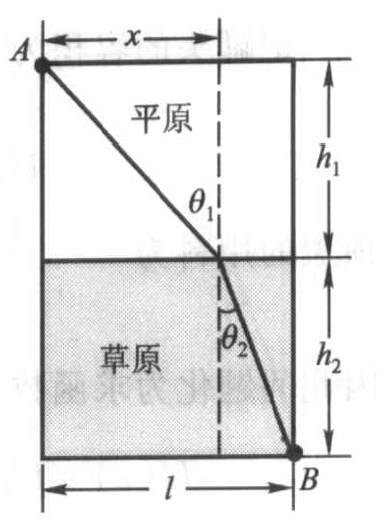
\includegraphics[width=0.8\textwidth]{light.png}
			\end{figure}
		\end{column}
	\end{columns}
\end{frame}

\begin{frame}
	\frametitle{基本计量经济学}

	\begin{block}{基本函数}
		1. 成本函数: 总成本函数 $C=C(Q)=C_0+C_1(Q)$, 其中 $Q$为产量, $C_0$ 为固定成本, $C_1(Q)$为变动成本; 平均成本函数 $\bar{C}=\frac{C(Q)}{Q}$.

		2. 需求函数 $Q=f(P)$, 其中 $P$ 为价格; 它的反函数 $\bar{P}=g(\bar{Q})$ 有时称为价格函数。

		3. 收益函数总收益函数 $R=R(P)=P \cdot Q=P \cdot f(P)$或 $\quad R=R(Q)=P \cdot Q=Q \cdot g(Q)$平均收益函数 $\bar{R}=\frac{R}{Q}$.

		4. 利润函数总利润函数 $L(Q)=R(Q)-C(Q)$.
	\end{block}
	\begin{block}{成本边际}
		边际成本: 成本函数 $C(Q)$ 的导数 $C^{\prime}(Q)$

		边际平均成本:平均成本 $\bar{C}(Q)$ 的导数
		$$
			\bar{C}^{\prime}(Q)=\left[\frac{C(Q)}{Q}\right]^{\prime}=\frac{Q C^{\prime}(Q)-C(Q)}{Q^2}
		$$
	\end{block}
\end{frame}

\begin{frame}
	\frametitle{基本计量经济学}
	\everymath{\displaystyle}
	\begin{block}{收益边际}
		边际收益: 收益函数 $R(Q)$ 的导数 $R^{\prime}(Q)$\\

		边际利润: 总利润函数 $L(Q)$ 的导数 $L^{\prime}(Q)=R^{\prime}(Q)-C^{\prime}(Q)$\\

		边际需求:  $f^{\prime}(P)=\frac{1}{\left[f^{-1}(Q)\right]^{\prime}}$
	\end{block}

	\begin{block}{弹性}
		一般的, 若函数 $y=f(x)$ 在区间内 $(a, b)$ 可导, 且 $f(x) \neq 0$, 则称 $\frac{E y}{E x}=\lim _{\Delta x \rightarrow 0} \frac{\Delta y / y}{\Delta x / x}=\lim _{\Delta x \rightarrow 0} \frac{\Delta y}{\Delta x} \cdot \frac{x}{y}=y^{\prime} \cdot \frac{x}{y}$ 为函数 $y=f(x)$ 在区间 $(a, b)$ 内的点弹性函数, 简称弹性函数.
	\end{block}
\end{frame}

% Thank you page
\beamertemplateshadingbackground{structure.fg!90}{structure.fg}
\begin{frame}[plain]
	\vfill
	\centering
	{
		\centering \Huge \color{white} Thank you for your attention!\\[10pt]Questions?
	}
	\vfill
\end{frame}


\end{document}


